\documentclass[handout]{beamer}
\usetheme{Madrid}
\usepackage{pdfpages}
\usepackage[utf8x]{inputenc}
\usepackage{url}
\usepackage{graphicx}
\usepackage{graphics}
\usepackage{adjustbox}
\usepackage{ragged2e}
\usepackage{amsmath, amssymb}
\usepackage{verbatim}
\usepackage{soul}
\usepackage{textpos}
\usepackage{xcolor}
\usepackage{tcolorbox}
\usepackage{lmodern,textcomp}
 \setbeamertemplate{enumerate items}[default]
 \setbeamertemplate{itemize items}[circle]
 \setbeamertemplate{frametitle continuation}{}
\setbeamertemplate{section in toc}[circle]
\setbeamertemplate{subsection in toc}[circle]

\usepackage{tabulary, booktabs}

\usepackage{hyperref}
\hypersetup{
    colorlinks=cyan,
    linkcolor=true,
    filecolor=cyan,      
    urlcolor=cyan,
}

\beamertemplatenavigationsymbolsempty

%%%%%%%%%%%%%%%Color%%%%%%%%%%%%%%%
\definecolor{KIPlum}{HTML}{880052}
\definecolor{box}{RGB}{250, 117, 144}
\usecolortheme[named=KIPlum]{structure}

%%%%%%%%%%%%%%%Bibliography setting%%%%%%%%%%%%%%%
\usepackage[numbers,comma,sort&compress]{natbib}
\makeatletter
\renewcommand{\@biblabel}[1]{#1.} %remove brackets from the ref list
\makeatother



%%%%%%%%%%%%%%%Title page%%%%%%%%%%%%%%%

\title[Applied Epi I: Interpreting results]{Applied Epidemiology I: Tables and interpreting results}
\date{\today}
\author[Enoch Yi-Tung Chen]{Enoch Yi-Tung Chen}
\institute[MEB]{Department of Medical Epidemiology and Biostatistics, Karolinska Insitutet}

%%%%%%%%%%%%%%\begin{document}%%%%%%%%%%%%%%%%

\begin{document}

\begin{frame}
\maketitle 
\end{frame}

%%%%%%%%%%%%%%Outline%%%%%%%%%%%%%%%%
\begin{frame}{Acknowledgements}
This course material is based on my learning from \href{https://staff.ki.se/people/analam}{Anastasia Lam}'s teachings in last year's Applied Epidemiology I lab sessions, and readings from \textit{Epidemiology} by Gordis \cite{Gordis2014}, \textit{A First Course in Probability and Statistics} by Goldsman and Goldsman \cite{Goldsman2020}, \textit{Principles of Biostatistics} by Pagano and Gauvreau \cite{Pagano2000}, and \textit{Biostatistics I} by Gabriel and Frumento \cite{Gabriel2020}. 

I especially want to thank Marlene Stratmann for reviewing the slides and Prof. Paul Dickman for providing me with suggestions to improving the teaching.

\end{frame}


%%%%%%%%%%%%%%Outline%%%%%%%%%%%%%%%%
\section*{Outline}
\begin{frame}{\secname}
 \begin{columns}[t]
        \begin{column}{.5\textwidth}
            \tableofcontents[sections={1-4}]
        \end{column}
        \begin{column}{.5\textwidth}
            \tableofcontents[sections={5-7}]
        \end{column}
\end{columns}
\end{frame}
%%%
\section{Tables}
\subsection{One-way tables}
\begin{frame}[fragile]{\secname: \subsecname}
\begin{itemize}	
	\item<1|handout:1-> We use cancer data still.
	\item<1|handout:1->[]
\begin{verbatim}
sysuse cancer, clear
keep if drug ==1 | drug == 2	
 \end{verbatim}
\item<2|handout:2-> One-way table of frequencies with mean and sd of age
\begin{verbatim}
. table died, contents(freq mean age sd age)

----------------------------------------------
1 if      |
patient   |
died      |      Freq.   mean(age)     sd(age)
----------+-----------------------------------
        0 |          9     55.1111    5.487359
        1 |         25       56.88    6.227091
----------------------------------------------


 \end{verbatim}

\end{itemize}
\end{frame}
%%%%%
\begin{frame}[fragile]{\secname: \subsecname}
\begin{itemize}	
\item One-way table of frequencies
\begin{verbatim}
. tabulate died

       1 if |
    patient |
       died |      Freq.     Percent        Cum.
------------+-----------------------------------
          0 |          9       26.47       26.47
          1 |         25       73.53      100.00
------------+-----------------------------------
      Total |         34      100.00
	
\end{verbatim}
\end{itemize}
\end{frame}

%%%%%
\begin{frame}[fragile]{\secname: \subsecname}
\begin{itemize}	
\item One-way tables of frequencies each variable specified
\scriptsize
\begin{verbatim}
. tab1 died drug
-> tabulation of died  

       1 if |
    patient |
       died |      Freq.     Percent        Cum.
------------+-----------------------------------
          0 |          9       26.47       26.47
          1 |         25       73.53      100.00
------------+-----------------------------------
      Total |         34      100.00

-> tabulation of drug  

  Drug type |
(1=placebo) |      Freq.     Percent        Cum.
------------+-----------------------------------
          0 |         14       41.18       41.18
          1 |         20       58.82      100.00
------------+-----------------------------------
      Total |         34      100.00


	
\end{verbatim}
\end{itemize}
\end{frame}

%%%
\begin{frame}[fragile]{\secname: \subsecname}
\begin{itemize}
\item Create table I of baseline characteristics using \verb|table1_mc|
\item This command is useful. Play it on your own!
\item See \verb|help table1_mc|
\end{itemize}
\scriptsize
\begin{verbatim}
. ssc install table1_mc, replace
. table1_mc, vars(age conts)
  +---------------------------------------------+
  |                                  Total      |
  |---------------------------------------------|
  |                                  N=34       |
  |---------------------------------------------|
  | Patient's age at start of exp.   56 (51-61) |
  +---------------------------------------------+
Data are presented as median (IQR).
\end{verbatim}
\end{frame}	

%%%
\subsection{Two by two tables}
\begin{frame}[fragile]{\secname: \subsecname}
\begin{itemize}
\item 2 by 2 table for drug and died with relative frequency by column or row
\end{itemize}
\scriptsize
\begin{verbatim}
. tabulate died drug, col row

      1 if |
   patient | Drug type (1=placebo)
      died |         0          1 |     Total
-----------+----------------------+----------
         0 |         8          1 |         9 
           |     88.89      11.11 |    100.00 
           |     57.14       5.00 |     26.47 
-----------+----------------------+----------
         1 |         6         19 |        25 
           |     24.00      76.00 |    100.00 
           |     42.86      95.00 |     73.53 
-----------+----------------------+----------
     Total |        14         20 |        34 
           |     41.18      58.82 |    100.00 
           |    100.00     100.00 |    100.00 
	
\end{verbatim}
\end{frame}	

%%%%
\begin{frame}[fragile]{\secname: \subsecname}
\begin{columns}[t]
\begin{column}{.6\textwidth}
\begin{itemize}
\item 2 by 2 table with chi-square test and fisher's exact test
\end{itemize}
\tiny
\begin{verbatim}
. tabulate died drug, col row chi2 exact
      1 if |
   patient | Drug type (1=placebo)
      died |         0          1 |     Total
-----------+----------------------+----------
         0 |         8          1 |         9 
           |     88.89      11.11 |    100.00 
           |     57.14       5.00 |     26.47 
-----------+----------------------+----------
         1 |         6         19 |        25 
           |     24.00      76.00 |    100.00 
           |     42.86      95.00 |     73.53 
-----------+----------------------+----------
     Total |        14         20 |        34 
           |     41.18      58.82 |    100.00 
           |    100.00     100.00 |    100.00 

          Pearson chi2(1) =  11.5039   Pr = 0.001
           Fisher's exact =                 0.001
\end{verbatim}
\end{column}
\begin{column}{.4\textwidth}
\begin{itemize}
\item<2|handout:2->How to interpret the results?
\item<3|handout:3-> Chi-square test: testing the association between two binary variables.
\item<4|handout:4> Using placebo has association with that the patients died or not.
\end{itemize}

\end{column}

\end{columns}

\end{frame}

%%%%
\begin{frame}[fragile]{\secname: \subsecname}

\begin{columns}
\begin{column}{.5\textwidth}
\begin{itemize}
\item 2 by 2 tables straitified by sex
\end{itemize}
\tiny
\begin{verbatim}
. bysort sex: tab died drug, col row chi2

-> sex = 0

      1 if |
   patient | Drug type (1=placebo)
      died |         0          1 |     Total
-----------+----------------------+----------
         0 |         6          1 |         7 
           |     85.71      14.29 |    100.00 
           |     75.00       9.09 |     36.84 
-----------+----------------------+----------
         1 |         2         10 |        12 
           |     16.67      83.33 |    100.00 
           |     25.00      90.91 |     63.16 
-----------+----------------------+----------
     Total |         8         11 |        19 
           |     42.11      57.89 |    100.00 
           |    100.00     100.00 |    100.00 

          Pearson chi2(1) =   8.6466   Pr = 0.003
\end{verbatim}
\end{column}

\begin{column}{.5\textwidth}
\tiny
\begin{verbatim}
-> sex = 1
      1 if |
   patient | Drug type (1=placebo)
      died |         0          1 |     Total
-----------+----------------------+----------
         0 |         2          0 |         2 
           |    100.00       0.00 |    100.00 
           |     33.33       0.00 |     13.33 
-----------+----------------------+----------
         1 |         4          9 |        13 
           |     30.77      69.23 |    100.00 
           |     66.67     100.00 |     86.67 
-----------+----------------------+----------
     Total |         6          9 |        15 
           |     40.00      60.00 |    100.00 
           |    100.00     100.00 |    100.00 

          Pearson chi2(1) =   3.4615   Pr = 0.063
\end{verbatim}
\end{column}
\end{columns}
\end{frame}

%%%%
\subsection{Stata tool for Epidemiology}
\begin{frame}{\secname: \subsecname}
\begin{itemize}
	\item How to use Stata to generate risk ratios (relative risk) and odds ratios?
	\item<2|handout:2-> A useful tool in Stata's default function can be found at 
	\item<2|handout:2-> Statistics - Epidemiology and related - Tables for epidemiologists
	\item[]<2|handout:2-> 
\includegraphics[scale=0.5]{image/bar}
	\item<3|handout:3> But before demonstrating how this works, a recapture on basic epi terms!
\end{itemize}

\end{frame}
%%%%
\section{Basic Epidemiology terms}
\subsection{Rate vs. proportion}
\begin{frame}{\secname: \subsecname}
\textbf{Rate}
\begin{itemize}
	  \item<2|handout:2-> Incidence (rate): $\frac{\text{no. of diseased}}{\text{total person-time}}$
	  \item<3|handout:3-> Mortality (rate): $\frac{\text{no. of deaths}}{\text{total person-time}}$
	  \item<4|handout:4-> Hazard (rate): in survival analysis, hazard is often defined as mortality rate.
	  \end{itemize}
\textbf{Proportion}
	\begin{itemize}
	\item<5|handout:5-> Cumulative incidence: \textbf{over a time period}, \begin{small}
 	$\frac{\text{no. of new cases of the disease}}{\text{no. of initially disease-free persons}}$
 \end{small}
	\item<6|handout:6-> Fatality: \textbf{over a time period}, $\frac{\text{no. of deaths of the disease}}{\text{no. of persons with the disease}}$
	\item<7|handout:7-> Point prevalence: \textbf{at a specified time}, $\frac{\text{no. of diseased}}{\text{no. of persons}}$
	\item<7|handout:7-> Period prevalence: \textbf{over a time period}, $\frac{\text{no. of diseased}}{\text{no. of persons}}$
	\item<8|handout:8-> Survival (proportion/probability) \st{rate}: \begin{center}
 	$\frac{\text{no. of alive persons (since diagnosis)}}{\text{no. of initially disease-free persons (since diagnosis)}}$
 \end{center}
	\end{itemize}
\textbf{Risk}
	\begin{itemize}
	\item<9|handout:9> Is risk a rate or a proportion?	
	\end{itemize}

\end{frame}
%%%
\begin{frame}{\secname: \subsecname}
\textbf{Quizs}
\begin{enumerate}
\item<2|handout:2->  What is the key difference between rate and proportion?
\begin{itemize}
	\item<3|handout:3-> TIME! 
	\item<3|handout:3-> Rate: person-time
	\item<3|handout:3-> Proportion: specify a period/point of time
\end{itemize}

\item<4|handout:4-> Mortality vs. fatality?
	\begin{itemize}
	\item<5|handout:5-> Mortality (rate): $\frac{\text{no. of deaths}}{\text{total person-time}}$
    \item<5|handout:5-> Fatality: over a time period, $\frac{\text{no. of deaths of the disease}}{\text{no. of persons with the disease}}$
 	
	\end{itemize}

\item<6|handout:6-> Is risk a rate or a proportion?

\end{enumerate}
\end{frame}

%%%%
\subsection{Risk, risk difference, risk ratio}
\begin{frame}{\secname: \subsecname}
	\textbf{Risk}: the proportion (probability) of an event, e.g., death. \\ 
	\begin{itemize}
		\item<2|handout:2-> Estimates of risk: cumulative incidence, cumulative hazard
		\item<3|handout:3-> E.g., in survival analysis, 

	\small
\[ \text{Cumulative hazard} = 1 - \text{Survival proportion} = \text{Cumulative probability of death}\] \\
	\[ F(t) = 1 - S(t) = P(T\leq t) \]
	\end{itemize}
\begin{itemize}
\normalsize
\item<4|handout:4-> Risk difference: the difference of the probabilities of an event between the exposed group and non-exposed group
\item<5|handout:5-> Risk ratio: the ratio of the probabilities of an event between the exposed group and non-exposed group
\item<6|handout:6> \textbf{Caution!} Relative risk could be either risk ratio or rate ratio! 
\end{itemize}
\end{frame}


%%
\begin{frame}{\secname: \subsecname}
\begin{columns}[t]
\begin{column}{0.5\textwidth}
\vspace{-10mm}
\begin{table}[h]
	\scriptsize
\begin{center}
\begin{tabular}{lccc}
\toprule
   & Female    & Male            & Total  \\ 
   & (Exposed) & (Unexposed)     &        \\ \midrule
shiba  & 2        & 2            & 4         \\
(Case) &          &              &           \\
guinea pig   & 2        & 1            & 3   \\
(Noncase) &          &              &           \\

Total  & 4        & 3            & 7     \\ \bottomrule
\end{tabular}
\end{center}
\end{table}

Epidemiologists love two by two tables!
\end{column}
    
\begin{column}{0.5\textwidth}
	\normalsize
	\begin{itemize}
		\item<2|handout:2-> Risk difference between females having shiba and males having shiba $= \widehat{p_F}- \widehat{p_M} = 2/4 - 2/3 -  = - 0.16667$
		\item<2|handout:2-> Interpretation: Females have 16.67 \% lower risk of having shiba than males. 
		\newline
		\item<3|handout:3> Risk ratio between females having shiba and males having shiba  $= \widehat{p_F} \div  \widehat{p_M} = 2/4 \div 2/3    = 0.75$.
		\item<3|handout:3> Interpretation: The RR of females having shiba is 0.75 times than males having shiba.

	\end{itemize}
\end{column}
    
\end{columns}
\end{frame}
%%%%

\subsection{Odds, odds ratio}
\begin{frame}{\secname: \subsecname}
	\textbf{Odds}: the ratio between those having and not having an outcome. \[ Odds = \frac{p}{1-p}\]
	
\begin{itemize}
\item<2|handout:2-> Odds ratio measures the association between an exposure and an outcome.
\[\text{Odds ratio (OR)} = \frac{Odds_{exposed}}{Odds_{unexposed}}\] \\  \item<3|handout:3-> E.g., the OR is $0.5$, which indicates that there is a 50\% decrease in the odds of having an outcome among the exposed compared to the unexposed.
\item<4|handout:4> Why there is no odds difference?
\end{itemize}
\end{frame}

%%%%

\begin{frame}{\secname: \subsecname}
\begin{columns}[t]

\begin{column}{0.5\textwidth}
\vspace{-10mm}
\begin{table}[h]
	\scriptsize
\begin{center}
\begin{tabular}{lccc}
\toprule
   & Female    & Male            & Total  \\ 
   & (Exposed) & (Unexposed)     &        \\ \midrule
shiba  & 2        & 2            & 4         \\
(Case) &          &              &           \\
guinea pig   & 2        & 1            & 3   \\
(Noncase) &          &              &           \\

Total  & 4        & 3            & 7     \\ \bottomrule
\end{tabular}
\end{center}
\end{table}

\begin{itemize}
	\normalsize
\item<2|handout:2-> The odds of having shiba among females is 
	\begin{displaymath}
		\scriptsize
	\begin{split}
			\widehat{odds_F} &=\frac{p(\text{having shiba}|\text{female})}{p(\text{having guinea pig}|\text{female})}\\
	                	&= \frac{(2/4) }{(2/4)} = 1
	\end{split}
		\end{displaymath}
\item<2|handout:2-> The odds of having shiba among males is 2 (calculation ignored).	
\end{itemize}
    \end{column}
    
	\begin{column}{0.5\textwidth}
	\normalsize
	\begin{itemize}
	\item<3|handout:3-> OR of having shiba \\ (females to males) 
	\item<3|handout:3-> OR = $\frac{Odds_{f}}{Odds_{m}}$ = $\frac{1}{2}$
	\item<4|handout:4> Interpretation: there is a 50\% decrease in the odds of having shiba among females compared to males. Higher odds of shiba ownership among males than females! 
	\item<4|handout:4> It seems that females instead love guinea pigs more.

	\end{itemize}

    	
    \end{column}
 \end{columns}
\end{frame}
%%%%
\section{Interpreting results}
\subsection{Principles}
\begin{frame}{\secname: \subsecname}
\begin{itemize}
\item When describing a ratio, it can ideally be illustrated by 
\begin{enumerate}
	\item \textcolor{red}{Exposed group}
	\item \colorbox{cyan}{Ratio} (exact value, higher or lower percentage)
	\item \colorbox{orange}{Outcome}
	\item \textcolor{blue}{Unexposed}
\end{enumerate}
\item<2|handout:2-> Example:
\begin{enumerate}
\item<2|handout:2-> \textcolor{red}{Females} have a \colorbox{cyan}{RR of 0.75	} \colorbox{orange}{having shiba} compared to \textcolor{blue}{males}.
\item<3|handout:3> \textcolor{red}{Females} have a \colorbox{cyan}{50\% decrease in the odds} of \colorbox{orange}{having shiba} compared to \textcolor{blue}{males}.
\end{enumerate}

\end{itemize}	
\end{frame}

%%%%
\subsection{Ratio $>$ or $<$ 1}
\begin{frame}{\secname: \subsecname}
\colorbox{cyan}{Ratio}
\begin{itemize}
\item<2|handout:2-> As ratio $<$ 1, 
	\begin{itemize}
			\item $(1-\text{RR}/\text{OR}) \times 100\% $
			\item E.g., RR $=$ 0.75, $(1-0.75) \times 100\% = 25\% $
			\item 25\% lower risk
	\end{itemize}
\item<3|handout:3> As ratio $>$ 1, 
	\begin{itemize}
			\item $(\text{RR}/\text{OR} - 1) \times 100\% $
			\item E.g., OR $=$ 2.05, $(2.05 - 1) \times 100\% = 105\% $
			\item The odds is 2 times higher.
			\item Twice the odds
	\end{itemize}

\end{itemize}
\end{frame}

%%%
\subsection{More examples}
\begin{frame}{\secname: \subsecname}
\footnotesize \textbf{Diabetes Is a Risk Factor for Pulmonary Tuberculosis: A Case-Control Study from Mwanza, Tanzania (Faurholt-Jepsen, 2011)}
\vspace{-3mm}
\begin{center}
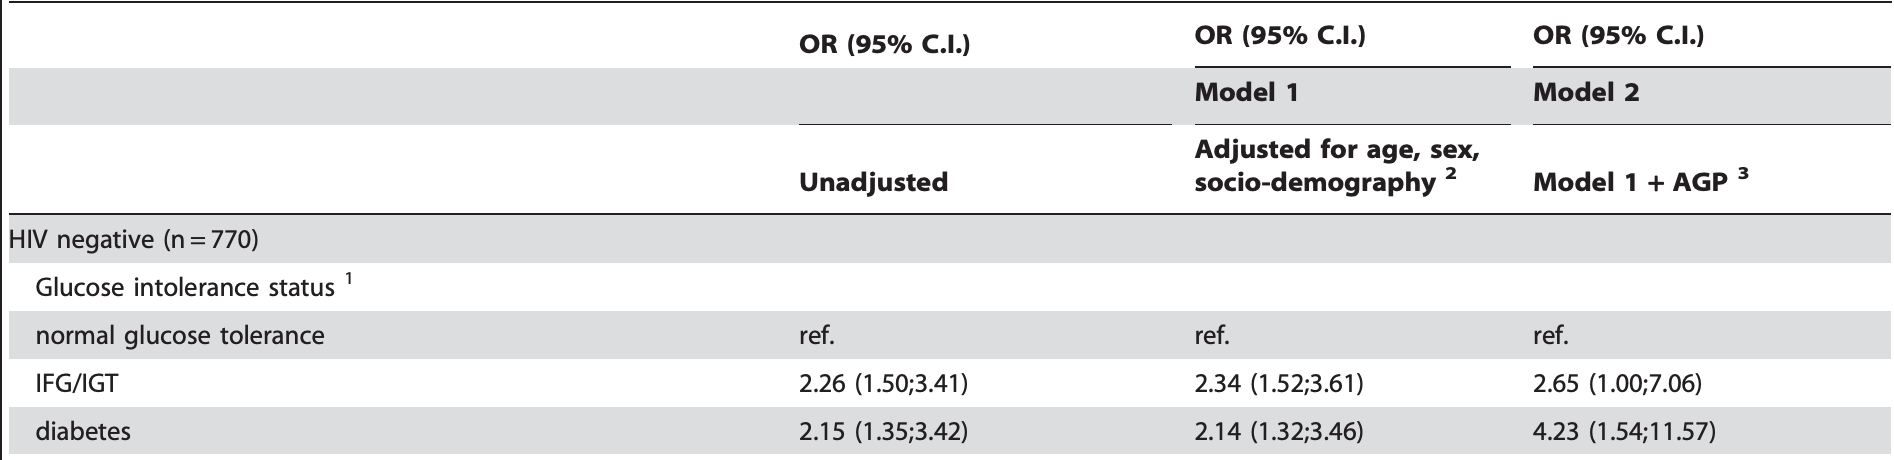
\includegraphics[scale=0.35]{image/dm_tb.png}
\end{center}
\begin{enumerate}
    \item<2|handout:2-> \textcolor{red}{People with diabetes} had a \colorbox{cyan}{higher odds} of \colorbox{orange}{TB} \colorbox{cyan}{(OR 2.15, 95\% CI: 1.35-3.42)} relative to \textcolor{blue}{people without diabetes}.
    \item<3|handout:3> \textcolor{red}{Having diabetes} was associated with more than a \colorbox{cyan}{2-fold increase (OR: 2.15, 95\% CI: 1.35; 3.42) in the odds} of \colorbox{orange}{TB} compared to \textcolor{blue}{not having diabetes}.
\end{enumerate}
\end{frame}

%%%
\begin{frame}{\secname: \subsecname}
\footnotesize \textbf{Bidirectional association between physical activity and symptoms of anxiety and depression: the Whitehall II study (Azevedo Da Silva, 2012)}
\begin{minipage}{0.45\textwidth}
\vspace{2mm}
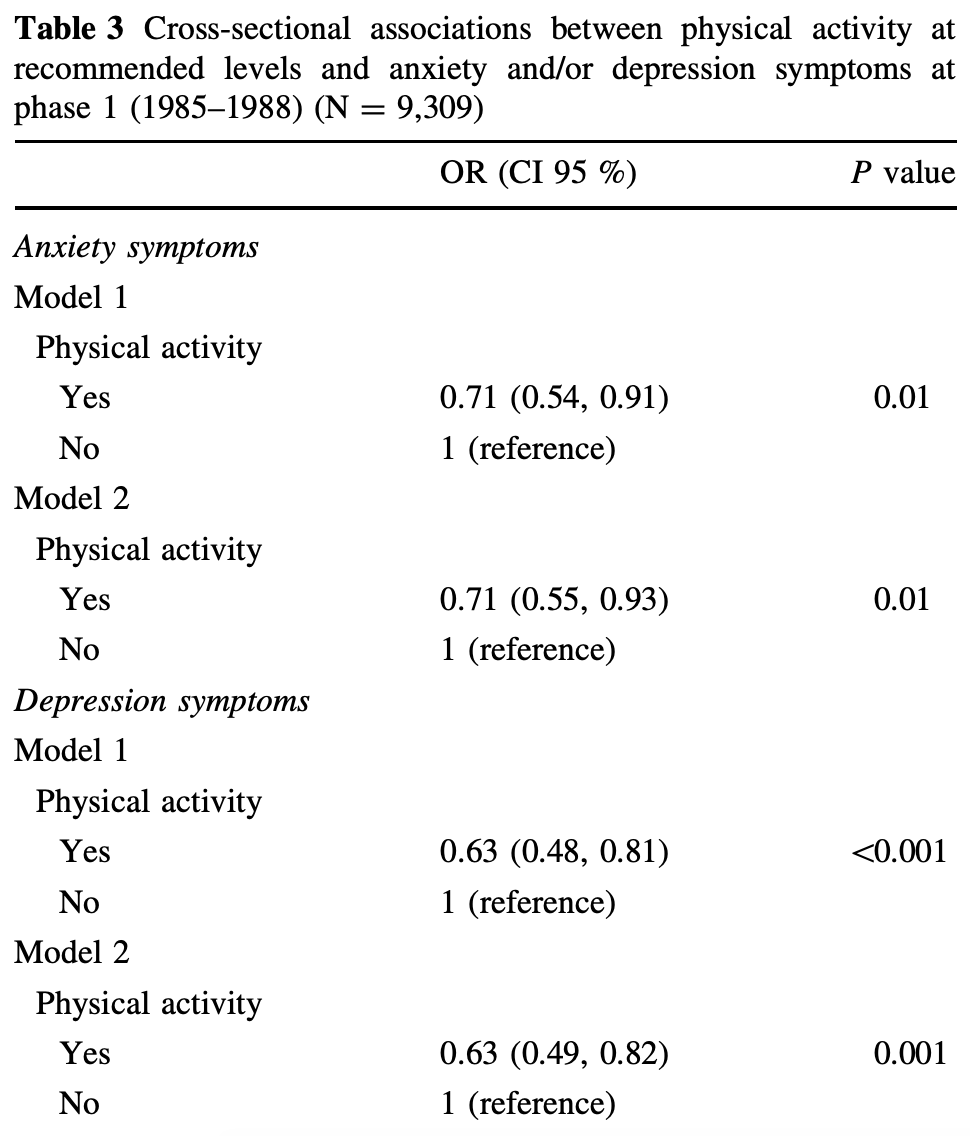
\includegraphics[scale=0.3]{image/physical.png}
\end{minipage}
\begin{minipage}{0.54\textwidth}
\begin{enumerate}
    \footnotesize
    \item<2|handout:2-> \textcolor{red}{Patients who conducted recommended levels of physical activity} had a \colorbox{cyan}{29\% lower odds} of \colorbox{orange}{anxiety}\colorbox{cyan}{(OR: 0.71, 95\% CI: 0.54-0.91)} and a \colorbox{cyan}{37\% lower odds} of \colorbox{orange}{depression} \colorbox{cyan}{(OR: 0.63, 95\% CI: 0.48-0.81)} relative to \textcolor{blue}{those who did not}.
    \item<3|handout:3> Our results showed that \textcolor{red}{individuals who practiced recommended levels of physical activity} were \colorbox{cyan}{less likely} to \colorbox{orange}{have anxiety} \colorbox{cyan}{(OR: 0.71, 95\% CI: 0.54-0.91)} and \colorbox{orange}{depression} \colorbox{cyan}{(OR: 0.63, 95\% CI: 0.48-0.81)} in comparison with \textcolor{blue}{those who did not}.
\end{enumerate}
\end{minipage}
\end{frame}



%%%
\section{Calculate ratios using Stata}
\subsection{Risk ratio}
\begin{frame}[fragile]{\secname: \subsecname}	
\begin{itemize}
\item Finally we come back to Stata again!
\item<2|handout:2> cs case exposed
\item[]<2|handout:2>\scriptsize \begin{verbatim}
. cs died drug

                 | Drug type [1=placebo]  |
                 |   Exposed   Unexposed  |      Total
-----------------+------------------------+-----------
           Cases |        19           6  |         25
        Noncases |         1           8  |          9
-----------------+------------------------+-----------
           Total |        20          14  |         34
                 |                        |
            Risk |       .95    .4285714  |   .7352941
                 |                        |
                 |      Point estimate    |    [95% Conf. Interval]
                 |------------------------+------------------------
 Risk difference |         .5214286       |     .245166    .7976911 
      Risk ratio |         2.216667       |    1.200631    4.092525 
 Attr. frac. ex. |         .5488722       |    .1671043    .7556521 
 Attr. frac. pop |         .4171429       |
                 +-------------------------------------------------
                               chi2(1) =    11.50  Pr>chi2 = 0.0007	
\end{verbatim}
\end{itemize}
\end{frame}

%%%%
\subsection{Odds ratio}
\begin{frame}[fragile]{\secname: \subsecname}	
\begin{itemize}
\item cs case exposed, or
\item[] \scriptsize \begin{verbatim}
. cs died drug, or

                 | Drug type [1=placebo]  |
                 |   Exposed   Unexposed  |      Total
-----------------+------------------------+-----------
           Cases |        19           6  |         25
        Noncases |         1           8  |          9
-----------------+------------------------+-----------
           Total |        20          14  |         34
                 |                        |
            Risk |       .95    .4285714  |   .7352941
                 |                        |
                 |      Point estimate    |    [95% Conf. Interval]
                 |------------------------+------------------------
 Risk difference |         .5214286       |     .245166    .7976911 
      Risk ratio |         2.216667       |    1.200631    4.092525 
 Attr. frac. ex. |         .5488722       |    .1671043    .7556521 
 Attr. frac. pop |         .4171429       |
      Odds ratio |         25.33333       |    3.189793           . (Cornfield)
                 +-------------------------------------------------
                               chi2(1) =    11.50  Pr>chi2 = 0.0007
 	
\end{verbatim}
\end{itemize}
\end{frame}

%%%%
\subsection{Incidence rate ratio}
\begin{frame}[fragile]{\secname: \subsecname}	
\begin{itemize}
\item ir case exposed studytime
\item[] \scriptsize \begin{verbatim}
 . ir died drug studytime
Incidence-rate comparison
                 | Drug type [1=placebo]  |
                 |   Exposed   Unexposed  |      Total
-----------------+------------------------+-----------
1 if patient die |        19           6  |         25
Months to death  |       180         209  |        389
-----------------+------------------------+-----------
                 |                        |
  Incidence rate |  .1055556    .0287081  |   .0642674
                 |                        |
                 |      Point estimate    |    [95% Conf. Interval]
                 |------------------------+------------------------
 Inc. rate diff. |         .0768474       |    .0241182    .1295766 
 Inc. rate ratio |         3.676852       |    1.411772    11.24864 (exact)
 Attr. frac. ex. |         .7280282       |    .2916701    .9111003 (exact)
 Attr. frac. pop |         .5533014       |
                 +-------------------------------------------------
Mid p-values for tests of incidence-rate difference:
  Adj Pr(Exposed 1 if patient die <= 19) = 0.9985 (lower one-sided)
  Adj Pr(Exposed 1 if patient die >= 19) = 0.0015 (upper one-sided)
                       Two-sided p-value = 0.0031
	
 \end{verbatim}
 \end{itemize}
\end{frame}

%%%
\section{References}
\begin{frame}[allowframebreaks,fragile]{\secname}
    \begin{scriptsize}
	\bibliographystyle{../bib/vancouv12}
	\bibliography{../bib/enochref.bib}
    \end{scriptsize}
\end{frame}



\end{document}